\documentclass[aspectratio=169,11pt]{beamer}
% =====================================================================
%  pds-beamer.tex — Estilo común de las transparencias.
%
%  Uso (desde teoría/Tx/transparencias/):
%     \documentclass[aspectratio=169,11pt]{beamer}
%     % =====================================================================
%  pds-beamer.tex — Estilo común de las transparencias.
%
%  Uso (desde teoría/Tx/transparencias/):
%     \documentclass[aspectratio=169,11pt]{beamer}
%     % =====================================================================
%  pds-beamer.tex — Estilo común de las transparencias.
%
%  Uso (desde teoría/Tx/transparencias/):
%     \documentclass[aspectratio=169,11pt]{beamer}
%     \input{../../comun/pds-beamer}
%     \title{...}  \subtitle{Tema x · ...}
%     \begin{document}
%       \portada
%       ...
%     \end{document}
%  Compilar con:  latexmk -xelatex  (o «make» desde teoría/)
% =====================================================================

\usetheme{Boadilla}
\usecolortheme{orchid}
\usefonttheme{professionalfonts}
\setbeamercovered{transparent}
\setbeamersize{text margin left=0.8cm, text margin right=0.8cm}
\setbeamertemplate{navigation symbols}{}
\setbeamertemplate{itemize item}[square]
\setbeamertemplate{itemize subitem}[circle]
\setbeamertemplate{itemize subsubitem}[triangle]
\setbeamertemplate{enumerate item}[square]
\setbeamertemplate{enumerate subitem}[circle]
\setbeamertemplate{caption}{\raggedright\insertcaption\par}

\input{../../comun/pds-comun.tex}

% Tipografía: Fira Sans + Fira Math (legibles en proyector)
\usepackage{fontspec}
\usepackage{unicode-math}
% Se cargan por nombre de fichero para que funcionen con cualquier
% instalación de TeX Live (o MiKTeX) sin instalar fuentes en el sistema.
\setmainfont{FiraSans}[Extension=.otf, UprightFont=*-Regular, BoldFont=*-SemiBold,
  ItalicFont=*-Italic, BoldItalicFont=*-SemiBoldItalic]
\setsansfont{FiraSans}[Extension=.otf, UprightFont=*-Regular, BoldFont=*-SemiBold,
  ItalicFont=*-Italic, BoldItalicFont=*-SemiBoldItalic]
\setmonofont{FiraMono}[Extension=.otf, UprightFont=*-Regular, BoldFont=*-Medium, AutoFakeSlant=0.15, Scale=0.92]
\setmathfont{FiraMath-Regular.otf}
\setmathfont{latinmodern-math.otf}[range={"229B,"22EE,"22F1}]

% Colores del tema ajustados a la paleta común (más contraste)
\setbeamercolor{structure}{fg=pdsazul}
\setbeamercolor{alerted text}{fg=pdsrojo}
\setbeamercolor{example text}{fg=pdsverde}
\setbeamercolor{block title}{bg=pdsazul, fg=white}
\setbeamercolor{block body}{bg=pdsfondo}
\setbeamercolor{block title alerted}{bg=pdsrojo, fg=white}
\setbeamercolor{block body alerted}{bg=pdsrojo!6}
\setbeamercolor{block title example}{bg=pdsverde, fg=white}
\setbeamercolor{block body example}{bg=pdsverde!6}
\setbeamercolor{frametitle}{fg=pdsazul, bg=white}
\setbeamerfont{frametitle}{size=\large, series=\bfseries}
\setbeamerfont{block title}{size=\normalsize, series=\bfseries}
\setbeamertemplate{blocks}[rounded][shadow=false]

% Logo en la esquina superior derecha de cada transparencia
\pgfdeclareimage[height=0.8cm]{logo}{../../comun/ucm.png}
\addtobeamertemplate{frametitle}{}{%
  \begin{tikzpicture}[remember picture, overlay]
    \node[anchor=north east, inner sep=0pt] at ([xshift=-0.25cm, yshift=-0.2cm]current page.north east) {\pgfuseimage{logo}};
  \end{tikzpicture}}

% Datos de portada
\author[\autorescorto]{\autores}
\institute[UCM]{\footnotesize\departamento\\\universidad}
\date[\curso]{\footnotesize\grado\\\curso}

\newcommand{\portada}{%
  \begin{frame}[plain]
    \begin{center}
      
\includegraphics[height=1.9cm]{../../comun/ucm.png}
    \end{center}
    \vspace{-0.4cm}
    \titlepage
  \end{frame}}

% Índice al empezar cada sección
\AtBeginSection[]{%
  \begin{frame}{Contenido}
    \tableofcontents[currentsection, hideothersubsections]
  \end{frame}}

\renewcommand{\pdscodesize}{\scriptsize}

% Utilidades
% \herramienta{T1-convolucion-continua}: enlace a la página publicada de
% herramientas/html (se abre en el navegador, sin instalar nada).
% \herramientaservidor{server/....py}: app que necesita Python (bokeh serve).
\newcommand{\urlherramientas}{https://ucm-237.github.io/PdS/}
\newcommand{\herramienta}[1]{%
  \par\vfill\hfill{\scriptsize\color{pdsgris}\faIcon\ \href{\urlherramientas#1.html}{Herramienta interactiva: \texttt{#1}}}}
\newcommand{\herramientaservidor}[1]{%
  \par\vfill\hfill{\scriptsize\color{pdsgris}\faIcon\ Herramienta interactiva (con Python): \texttt{herramientas/#1}}}
\newcommand{\faIcon}{\textbf{▶}}
\newcommand{\gris}[1]{{\color{pdsgris}#1}}
\newcommand{\nota}[1]{\par\vspace{2pt}{\footnotesize\color{pdsgris}\textit{#1}}\par}
% Nota sobre una errata de versiones anteriores (solo con \ERRATAS)
\newcommand{\errata}[1]{\iferratas\nota{Errata de versiones anteriores: #1}\fi}
\newcommand{\apuntes}[1]{\nota{Más detalle en los apuntes, #1.}}

% Bloques con nombre en castellano
\newenvironment{definicion}[1][Definición]{\begin{block}{#1}}{\end{block}}
\newenvironment{importante}[1][Importante]{\begin{alertblock}{#1}}{\end{alertblock}}
\newenvironment{ejemplo}[1][Ejemplo]{\begin{exampleblock}{#1}}{\end{exampleblock}}

%     \title{...}  \subtitle{Tema x · ...}
%     \begin{document}
%       \portada
%       ...
%     \end{document}
%  Compilar con:  latexmk -xelatex  (o «make» desde teoría/)
% =====================================================================

\usetheme{Boadilla}
\usecolortheme{orchid}
\usefonttheme{professionalfonts}
\setbeamercovered{transparent}
\setbeamersize{text margin left=0.8cm, text margin right=0.8cm}
\setbeamertemplate{navigation symbols}{}
\setbeamertemplate{itemize item}[square]
\setbeamertemplate{itemize subitem}[circle]
\setbeamertemplate{itemize subsubitem}[triangle]
\setbeamertemplate{enumerate item}[square]
\setbeamertemplate{enumerate subitem}[circle]
\setbeamertemplate{caption}{\raggedright\insertcaption\par}

% =====================================================================
%  pds-comun.tex — Paquetes, colores y estilos de código comunes a
%  transparencias, apuntes y hojas de ejercicios. Compilar con XeLaTeX.
%  No cargar directamente: lo cargan pds-beamer.tex y pds-apuntes.tex.
% =====================================================================

\usepackage{polyglossia}
\setmainlanguage{spanish}
\usepackage{mathtools}
\usepackage{graphicx}
\usepackage{booktabs}
\usepackage{multirow}
\usepackage{array}
\usepackage{xcolor}
\usepackage{tikz}
\usetikzlibrary{positioning,arrows.meta,calc,shapes.geometric,decorations.pathreplacing}
\usepackage{listings}
\usepackage{siunitx}
\sisetup{output-decimal-marker={,}, group-separator={\,}, per-mode=symbol}

% Notas de erratas de versiones anteriores: no se imprimen salvo que se
% defina \ERRATAS antes de cargar el estilo (make ERRATAS=1)
\newif\iferratas
\ifdefined\ERRATAS \erratastrue \fi

% Ruta común (logo y figuras compartidas)
\providecommand{\rutacomun}{../../comun/}
\input{\rutacomun datos.tex}

% ---------------------------------------------------------------------
%  Paleta (la misma que usan las figuras generadas con Python,
%  ver comun/pds_estilo.py)
% ---------------------------------------------------------------------
\definecolor{pdsazul}{HTML}{2B3A8C}
\definecolor{pdsrojo}{HTML}{C0392B}
\definecolor{pdsverde}{HTML}{1E7B4F}
\definecolor{pdsnaranja}{HTML}{D9822B}
\definecolor{pdsgris}{HTML}{5A5A66}
\definecolor{pdsfondo}{HTML}{F3F4FA}
\definecolor{pdscodigo}{HTML}{F7F7F2}

% ---------------------------------------------------------------------
%  Diagramas de bloques (TikZ)
% ---------------------------------------------------------------------
\tikzset{
  bloque/.style={rectangle, rounded corners=2pt, draw=pdsazul!80, fill=pdsfondo,
                 very thick, minimum height=8mm, minimum width=14mm, align=center},
  sumador/.style={circle, draw=pdsazul!80, fill=pdsfondo, thick, inner sep=1.5pt},
  flecha/.style={-{Stealth[length=2.2mm]}, thick, pdsgris},
}

% ---------------------------------------------------------------------
%  Código: Python y Matlab en paralelo
% ---------------------------------------------------------------------
\newcommand{\pdscodesize}{\footnotesize}
\lstdefinestyle{pds}{
  basicstyle=\ttfamily\pdscodesize,
  keywordstyle=\color{pdsazul}\bfseries,
  commentstyle=\color{pdsverde}\itshape,
  stringstyle=\color{pdsrojo},
  numbers=none,
  backgroundcolor=\color{pdscodigo},
  frame=single, rulecolor=\color{pdsgris!40}, framerule=0.4pt,
  xleftmargin=2pt, xrightmargin=2pt, aboveskip=2pt, belowskip=2pt,
  columns=fullflexible, keepspaces=true,
  showstringspaces=false, breaklines=true, tabsize=4,
  upquote=true,
  % Con XeLaTeX, listings desordena los caracteres no ASCII junto a
  % dígitos («2π» sale «π2»): se sustituyen por su versión matemática.
  literate={π}{{$\pi$}}1 {δ}{{$\delta$}}1 {ω}{{$\omega$}}1 {Ω}{{$\Omega$}}1
           {≈}{{$\approx$}}1 {µ}{{$\mu$}}1 {·}{{$\cdot$}}1 {α}{{$\alpha$}}1
           {á}{{á}}1 {é}{{é}}1 {í}{{í}}1 {ó}{{ó}}1 {ú}{{ú}}1 {ñ}{{ñ}}1 {¿}{{¿}}1,
}
\lstdefinestyle{python}{style=pds, language=Python,
  morekeywords={as,True,False,None}}
\lstdefinestyle{matlab}{style=pds, language=Matlab,
  morekeywords={function,end,true,false}}

% \codigo{<ruta sin extensión>} muestra el mismo ejemplo en Python
% y en Matlab, uno al lado del otro. Los ficheros viven en
% ../codigo/python/<nombre>.py y ../codigo/matlab/<nombre>.m y se
% ejecutan en las pruebas (make prueba-codigo).
\newcommand{\rutacodigo}{../codigo/}
\newcommand{\codigoetiqueta}[1]{{\sffamily\scriptsize\bfseries\color{pdsgris}#1}}
\newcommand{\codigo}[2][]{%
  \par\noindent
  \begin{minipage}[t]{0.495\linewidth}
    \codigoetiqueta{Python}\par\vspace{1pt}
    \lstinputlisting[style=python,#1]{\rutacodigo python/#2.py}
  \end{minipage}\hfill
  \begin{minipage}[t]{0.495\linewidth}
    \codigoetiqueta{Matlab}\par\vspace{1pt}
    \lstinputlisting[style=matlab,#1]{\rutacodigo matlab/#2.m}
  \end{minipage}\par}

\input{\rutacomun notacion.tex}


% Tipografía: Fira Sans + Fira Math (legibles en proyector)
\usepackage{fontspec}
\usepackage{unicode-math}
% Se cargan por nombre de fichero para que funcionen con cualquier
% instalación de TeX Live (o MiKTeX) sin instalar fuentes en el sistema.
\setmainfont{FiraSans}[Extension=.otf, UprightFont=*-Regular, BoldFont=*-SemiBold,
  ItalicFont=*-Italic, BoldItalicFont=*-SemiBoldItalic]
\setsansfont{FiraSans}[Extension=.otf, UprightFont=*-Regular, BoldFont=*-SemiBold,
  ItalicFont=*-Italic, BoldItalicFont=*-SemiBoldItalic]
\setmonofont{FiraMono}[Extension=.otf, UprightFont=*-Regular, BoldFont=*-Medium, AutoFakeSlant=0.15, Scale=0.92]
\setmathfont{FiraMath-Regular.otf}
\setmathfont{latinmodern-math.otf}[range={"229B,"22EE,"22F1}]

% Colores del tema ajustados a la paleta común (más contraste)
\setbeamercolor{structure}{fg=pdsazul}
\setbeamercolor{alerted text}{fg=pdsrojo}
\setbeamercolor{example text}{fg=pdsverde}
\setbeamercolor{block title}{bg=pdsazul, fg=white}
\setbeamercolor{block body}{bg=pdsfondo}
\setbeamercolor{block title alerted}{bg=pdsrojo, fg=white}
\setbeamercolor{block body alerted}{bg=pdsrojo!6}
\setbeamercolor{block title example}{bg=pdsverde, fg=white}
\setbeamercolor{block body example}{bg=pdsverde!6}
\setbeamercolor{frametitle}{fg=pdsazul, bg=white}
\setbeamerfont{frametitle}{size=\large, series=\bfseries}
\setbeamerfont{block title}{size=\normalsize, series=\bfseries}
\setbeamertemplate{blocks}[rounded][shadow=false]

% Logo en la esquina superior derecha de cada transparencia
\pgfdeclareimage[height=0.8cm]{logo}{../../comun/ucm.png}
\addtobeamertemplate{frametitle}{}{%
  \begin{tikzpicture}[remember picture, overlay]
    \node[anchor=north east, inner sep=0pt] at ([xshift=-0.25cm, yshift=-0.2cm]current page.north east) {\pgfuseimage{logo}};
  \end{tikzpicture}}

% Datos de portada
\author[\autorescorto]{\autores}
\institute[UCM]{\footnotesize\departamento\\\universidad}
\date[\curso]{\footnotesize\grado\\\curso}

\newcommand{\portada}{%
  \begin{frame}[plain]
    \begin{center}
      
\includegraphics[height=1.9cm]{../../comun/ucm.png}
    \end{center}
    \vspace{-0.4cm}
    \titlepage
  \end{frame}}

% Índice al empezar cada sección
\AtBeginSection[]{%
  \begin{frame}{Contenido}
    \tableofcontents[currentsection, hideothersubsections]
  \end{frame}}

\renewcommand{\pdscodesize}{\scriptsize}

% Utilidades
% \herramienta{T1-convolucion-continua}: enlace a la página publicada de
% herramientas/html (se abre en el navegador, sin instalar nada).
% \herramientaservidor{server/....py}: app que necesita Python (bokeh serve).
\newcommand{\urlherramientas}{https://ucm-237.github.io/PdS/}
\newcommand{\herramienta}[1]{%
  \par\vfill\hfill{\scriptsize\color{pdsgris}\faIcon\ \href{\urlherramientas#1.html}{Herramienta interactiva: \texttt{#1}}}}
\newcommand{\herramientaservidor}[1]{%
  \par\vfill\hfill{\scriptsize\color{pdsgris}\faIcon\ Herramienta interactiva (con Python): \texttt{herramientas/#1}}}
\newcommand{\faIcon}{\textbf{▶}}
\newcommand{\gris}[1]{{\color{pdsgris}#1}}
\newcommand{\nota}[1]{\par\vspace{2pt}{\footnotesize\color{pdsgris}\textit{#1}}\par}
% Nota sobre una errata de versiones anteriores (solo con \ERRATAS)
\newcommand{\errata}[1]{\iferratas\nota{Errata de versiones anteriores: #1}\fi}
\newcommand{\apuntes}[1]{\nota{Más detalle en los apuntes, #1.}}

% Bloques con nombre en castellano
\newenvironment{definicion}[1][Definición]{\begin{block}{#1}}{\end{block}}
\newenvironment{importante}[1][Importante]{\begin{alertblock}{#1}}{\end{alertblock}}
\newenvironment{ejemplo}[1][Ejemplo]{\begin{exampleblock}{#1}}{\end{exampleblock}}

%     \title{...}  \subtitle{Tema x · ...}
%     \begin{document}
%       \portada
%       ...
%     \end{document}
%  Compilar con:  latexmk -xelatex  (o «make» desde teoría/)
% =====================================================================

\usetheme{Boadilla}
\usecolortheme{orchid}
\usefonttheme{professionalfonts}
\setbeamercovered{transparent}
\setbeamersize{text margin left=0.8cm, text margin right=0.8cm}
\setbeamertemplate{navigation symbols}{}
\setbeamertemplate{itemize item}[square]
\setbeamertemplate{itemize subitem}[circle]
\setbeamertemplate{itemize subsubitem}[triangle]
\setbeamertemplate{enumerate item}[square]
\setbeamertemplate{enumerate subitem}[circle]
\setbeamertemplate{caption}{\raggedright\insertcaption\par}

% =====================================================================
%  pds-comun.tex — Paquetes, colores y estilos de código comunes a
%  transparencias, apuntes y hojas de ejercicios. Compilar con XeLaTeX.
%  No cargar directamente: lo cargan pds-beamer.tex y pds-apuntes.tex.
% =====================================================================

\usepackage{polyglossia}
\setmainlanguage{spanish}
\usepackage{mathtools}
\usepackage{graphicx}
\usepackage{booktabs}
\usepackage{multirow}
\usepackage{array}
\usepackage{xcolor}
\usepackage{tikz}
\usetikzlibrary{positioning,arrows.meta,calc,shapes.geometric,decorations.pathreplacing}
\usepackage{listings}
\usepackage{siunitx}
\sisetup{output-decimal-marker={,}, group-separator={\,}, per-mode=symbol}

% Notas de erratas de versiones anteriores: no se imprimen salvo que se
% defina \ERRATAS antes de cargar el estilo (make ERRATAS=1)
\newif\iferratas
\ifdefined\ERRATAS \erratastrue \fi

% Ruta común (logo y figuras compartidas)
\providecommand{\rutacomun}{../../comun/}
\input{\rutacomun datos.tex}

% ---------------------------------------------------------------------
%  Paleta (la misma que usan las figuras generadas con Python,
%  ver comun/pds_estilo.py)
% ---------------------------------------------------------------------
\definecolor{pdsazul}{HTML}{2B3A8C}
\definecolor{pdsrojo}{HTML}{C0392B}
\definecolor{pdsverde}{HTML}{1E7B4F}
\definecolor{pdsnaranja}{HTML}{D9822B}
\definecolor{pdsgris}{HTML}{5A5A66}
\definecolor{pdsfondo}{HTML}{F3F4FA}
\definecolor{pdscodigo}{HTML}{F7F7F2}

% ---------------------------------------------------------------------
%  Diagramas de bloques (TikZ)
% ---------------------------------------------------------------------
\tikzset{
  bloque/.style={rectangle, rounded corners=2pt, draw=pdsazul!80, fill=pdsfondo,
                 very thick, minimum height=8mm, minimum width=14mm, align=center},
  sumador/.style={circle, draw=pdsazul!80, fill=pdsfondo, thick, inner sep=1.5pt},
  flecha/.style={-{Stealth[length=2.2mm]}, thick, pdsgris},
}

% ---------------------------------------------------------------------
%  Código: Python y Matlab en paralelo
% ---------------------------------------------------------------------
\newcommand{\pdscodesize}{\footnotesize}
\lstdefinestyle{pds}{
  basicstyle=\ttfamily\pdscodesize,
  keywordstyle=\color{pdsazul}\bfseries,
  commentstyle=\color{pdsverde}\itshape,
  stringstyle=\color{pdsrojo},
  numbers=none,
  backgroundcolor=\color{pdscodigo},
  frame=single, rulecolor=\color{pdsgris!40}, framerule=0.4pt,
  xleftmargin=2pt, xrightmargin=2pt, aboveskip=2pt, belowskip=2pt,
  columns=fullflexible, keepspaces=true,
  showstringspaces=false, breaklines=true, tabsize=4,
  upquote=true,
  % Con XeLaTeX, listings desordena los caracteres no ASCII junto a
  % dígitos («2π» sale «π2»): se sustituyen por su versión matemática.
  literate={π}{{$\pi$}}1 {δ}{{$\delta$}}1 {ω}{{$\omega$}}1 {Ω}{{$\Omega$}}1
           {≈}{{$\approx$}}1 {µ}{{$\mu$}}1 {·}{{$\cdot$}}1 {α}{{$\alpha$}}1
           {á}{{á}}1 {é}{{é}}1 {í}{{í}}1 {ó}{{ó}}1 {ú}{{ú}}1 {ñ}{{ñ}}1 {¿}{{¿}}1,
}
\lstdefinestyle{python}{style=pds, language=Python,
  morekeywords={as,True,False,None}}
\lstdefinestyle{matlab}{style=pds, language=Matlab,
  morekeywords={function,end,true,false}}

% \codigo{<ruta sin extensión>} muestra el mismo ejemplo en Python
% y en Matlab, uno al lado del otro. Los ficheros viven en
% ../codigo/python/<nombre>.py y ../codigo/matlab/<nombre>.m y se
% ejecutan en las pruebas (make prueba-codigo).
\newcommand{\rutacodigo}{../codigo/}
\newcommand{\codigoetiqueta}[1]{{\sffamily\scriptsize\bfseries\color{pdsgris}#1}}
\newcommand{\codigo}[2][]{%
  \par\noindent
  \begin{minipage}[t]{0.495\linewidth}
    \codigoetiqueta{Python}\par\vspace{1pt}
    \lstinputlisting[style=python,#1]{\rutacodigo python/#2.py}
  \end{minipage}\hfill
  \begin{minipage}[t]{0.495\linewidth}
    \codigoetiqueta{Matlab}\par\vspace{1pt}
    \lstinputlisting[style=matlab,#1]{\rutacodigo matlab/#2.m}
  \end{minipage}\par}

\input{\rutacomun notacion.tex}


% Tipografía: Fira Sans + Fira Math (legibles en proyector)
\usepackage{fontspec}
\usepackage{unicode-math}
% Se cargan por nombre de fichero para que funcionen con cualquier
% instalación de TeX Live (o MiKTeX) sin instalar fuentes en el sistema.
\setmainfont{FiraSans}[Extension=.otf, UprightFont=*-Regular, BoldFont=*-SemiBold,
  ItalicFont=*-Italic, BoldItalicFont=*-SemiBoldItalic]
\setsansfont{FiraSans}[Extension=.otf, UprightFont=*-Regular, BoldFont=*-SemiBold,
  ItalicFont=*-Italic, BoldItalicFont=*-SemiBoldItalic]
\setmonofont{FiraMono}[Extension=.otf, UprightFont=*-Regular, BoldFont=*-Medium, AutoFakeSlant=0.15, Scale=0.92]
\setmathfont{FiraMath-Regular.otf}
\setmathfont{latinmodern-math.otf}[range={"229B,"22EE,"22F1}]

% Colores del tema ajustados a la paleta común (más contraste)
\setbeamercolor{structure}{fg=pdsazul}
\setbeamercolor{alerted text}{fg=pdsrojo}
\setbeamercolor{example text}{fg=pdsverde}
\setbeamercolor{block title}{bg=pdsazul, fg=white}
\setbeamercolor{block body}{bg=pdsfondo}
\setbeamercolor{block title alerted}{bg=pdsrojo, fg=white}
\setbeamercolor{block body alerted}{bg=pdsrojo!6}
\setbeamercolor{block title example}{bg=pdsverde, fg=white}
\setbeamercolor{block body example}{bg=pdsverde!6}
\setbeamercolor{frametitle}{fg=pdsazul, bg=white}
\setbeamerfont{frametitle}{size=\large, series=\bfseries}
\setbeamerfont{block title}{size=\normalsize, series=\bfseries}
\setbeamertemplate{blocks}[rounded][shadow=false]

% Logo en la esquina superior derecha de cada transparencia
\pgfdeclareimage[height=0.8cm]{logo}{../../comun/ucm.png}
\addtobeamertemplate{frametitle}{}{%
  \begin{tikzpicture}[remember picture, overlay]
    \node[anchor=north east, inner sep=0pt] at ([xshift=-0.25cm, yshift=-0.2cm]current page.north east) {\pgfuseimage{logo}};
  \end{tikzpicture}}

% Datos de portada
\author[\autorescorto]{\autores}
\institute[UCM]{\footnotesize\departamento\\\universidad}
\date[\curso]{\footnotesize\grado\\\curso}

\newcommand{\portada}{%
  \begin{frame}[plain]
    \begin{center}
      
\includegraphics[height=1.9cm]{../../comun/ucm.png}
    \end{center}
    \vspace{-0.4cm}
    \titlepage
  \end{frame}}

% Índice al empezar cada sección
\AtBeginSection[]{%
  \begin{frame}{Contenido}
    \tableofcontents[currentsection, hideothersubsections]
  \end{frame}}

\renewcommand{\pdscodesize}{\scriptsize}

% Utilidades
% \herramienta{T1-convolucion-continua}: enlace a la página publicada de
% herramientas/html (se abre en el navegador, sin instalar nada).
% \herramientaservidor{server/....py}: app que necesita Python (bokeh serve).
\newcommand{\urlherramientas}{https://ucm-237.github.io/PdS/}
\newcommand{\herramienta}[1]{%
  \par\vfill\hfill{\scriptsize\color{pdsgris}\faIcon\ \href{\urlherramientas#1.html}{Herramienta interactiva: \texttt{#1}}}}
\newcommand{\herramientaservidor}[1]{%
  \par\vfill\hfill{\scriptsize\color{pdsgris}\faIcon\ Herramienta interactiva (con Python): \texttt{herramientas/#1}}}
\newcommand{\faIcon}{\textbf{▶}}
\newcommand{\gris}[1]{{\color{pdsgris}#1}}
\newcommand{\nota}[1]{\par\vspace{2pt}{\footnotesize\color{pdsgris}\textit{#1}}\par}
% Nota sobre una errata de versiones anteriores (solo con \ERRATAS)
\newcommand{\errata}[1]{\iferratas\nota{Errata de versiones anteriores: #1}\fi}
\newcommand{\apuntes}[1]{\nota{Más detalle en los apuntes, #1.}}

% Bloques con nombre en castellano
\newenvironment{definicion}[1][Definición]{\begin{block}{#1}}{\end{block}}
\newenvironment{importante}[1][Importante]{\begin{alertblock}{#1}}{\end{alertblock}}
\newenvironment{ejemplo}[1][Ejemplo]{\begin{exampleblock}{#1}}{\end{exampleblock}}

\graphicspath{{../figuras/}}

\title[T2 · Muestreo]{Muestreo y reconstrucción de señales}
\subtitle{Tema 2 · Parte 1: conversión A/D y muestreo periódico}

\begin{document}
\portada

% =====================================================================
\begin{frame}{Objetivos del tema}
  \begin{columns}[T]
    \begin{column}{0.52\textwidth}
      Entender y caracterizar matemáticamente el paso entre el mundo continuo y el discreto:
      \begin{itemize}
        \item Conversores A/D y D/A.
        \item Muestreo periódico: \alert{aliasing} y teorema de Nyquist–Shannon.
        \item Reconstrucción ideal y con retenedores.
        \item Cuantificación y codificación.
        \item Cambio de la frecuencia de muestreo de una señal discreta.
      \end{itemize}
    \end{column}
    \begin{column}{0.44\textwidth}
      \begin{block}{Material del tema}
        \small
        \begin{enumerate}
          \item Conversión A/D y muestreo periódico
          \item Reconstrucción
          \item Cuantificación y codificación
          \item Muestreo de señales discretas
        \end{enumerate}
        \smallskip
        Apuntes, hoja de ejercicios y ejemplos en Python y Matlab.
      \end{block}
    \end{column}
  \end{columns}
\end{frame}

% =====================================================================
\section{Conversión analógico-digital}

\begin{frame}{Procesado analógico y procesado digital}
  \begin{columns}[T]
    \begin{column}{0.48\textwidth}
      \alert{Procesadores analógicos}
      \begin{itemize}\small
        \item Predictor de mareas de Lord Kelvin (1873).
        \item Moduladores y demoduladores, filtros $RLC$.
        \item Amplificadores operacionales (años 40): suman, integran, derivan, filtran.
        \item Rápidos, pero sensibles al ruido y a la deriva de los componentes, y poco flexibles.
      \end{itemize}
    \end{column}
    \begin{column}{0.48\textwidth}
      \alert{Procesado digital}
      \begin{itemize}\small
        \item 1965: Cooley y Tukey publican la FFT \gris{(Gauss ya había usado una idea parecida hacia 1805).}
        \item 1979: Intel 2920, procesador analógico de señal con núcleo digital.
        \item 1983: Texas Instruments TMS32010, primer DSP de gran difusión: arquitectura Harvard y operación MAC (multiplicar y acumular) en un ciclo.
        \item Flexible y repetible; a cambio, ancho de banda limitado por $f_s$, cuantificación y latencia.
      \end{itemize}
    \end{column}
  \end{columns}
\end{frame}

\begin{frame}{La cadena de procesado digital}
  \begin{center}
    \resizebox{\linewidth}{!}{%
    \begin{tikzpicture}[node distance=1.0cm]
      \node (x) {$x(t)$};
      \node[bloque, right=of x] (aa) {Filtro\\antialiasing};
      \node[bloque, right=of aa] (ad) {A/D};
      \node[bloque, right=of ad, fill=pdsazul!12] (dsp) {Procesado\\digital};
      \node[bloque, right=of dsp] (da) {D/A};
      \node[bloque, right=of da] (rec) {Filtro de\\reconstrucción};
      \node[right=of rec] (y) {$y(t)$};
      \draw[flecha] (x) -- (aa);
      \draw[flecha] (aa) -- node[above, font=\footnotesize]{$x_a(t)$} (ad);
      \draw[flecha] (ad) -- node[above, font=\footnotesize]{$x[n]$} (dsp);
      \draw[flecha] (dsp) -- node[above, font=\footnotesize]{$y[n]$} (da);
      \draw[flecha] (da) -- node[above, font=\footnotesize]{$y_a(t)$} (rec);
      \draw[flecha] (rec) -- (y);
    \end{tikzpicture}}
  \end{center}
  \begin{itemize}\small
    \item \alert{Filtro antialiasing}: limita el ancho de banda de la señal antes de muestrear (parte 1).
    \item \alert{A/D}: muestrea, cuantifica y codifica (partes 1 y 3).
    \item \alert{Procesado digital}: el algoritmo (temas 3 a 6).
    \item \alert{D/A} y \alert{filtro de reconstrucción} (o de suavizado): devuelven una señal continua y eliminan las altas frecuencias que introduce la reconstrucción (parte 2).
  \end{itemize}
\end{frame}

\begin{frame}{Muestreo, cuantificación y codificación}
  \begin{center}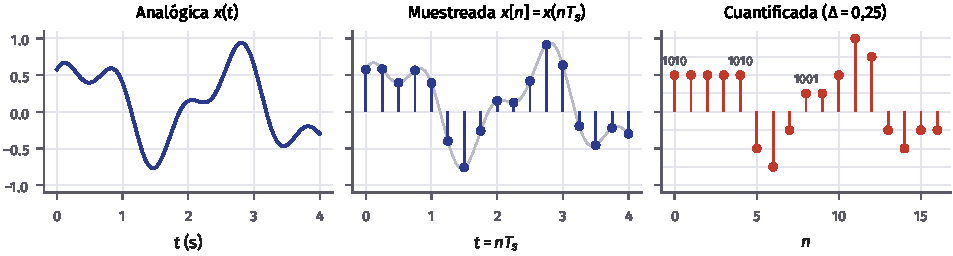
\includegraphics[width=0.92\linewidth]{muestreo_cuant_cod}\end{center}
  \begin{itemize}\small
    \item \alert{Muestreo}: se toman valores de $x(t)$ en instantes discretos, $x[n]=x(nT_s)$. Tiempo discreto, amplitud continua.
    \item \alert{Cuantificación}: cada muestra se aproxima por uno de un número finito de niveles. Amplitud discreta: señal digital.
    \item \alert{Codificación}: cada nivel se representa con una palabra de $b$ bits.
  \end{itemize}
  \nota{En un conversor real, un circuito de muestreo y retención (\emph{sample and hold}) congela la tensión mientras el cuantificador la convierte.}
\end{frame}

% =====================================================================
\section{Muestreo periódico}

\begin{frame}{Muestreo periódico}
  \begin{definicion}[Muestreo periódico o uniforme]
    \[
      x[n]=x(nT_s),\qquad n\in\Z
    \]
    $T_s$: \alert{periodo de muestreo}; \ $f_s=1/T_s$: \alert{frecuencia de muestreo} (Hz); \ $\omega_s=2\pi f_s=2\pi/T_s$ (rad/s).
  \end{definicion}
  \begin{center}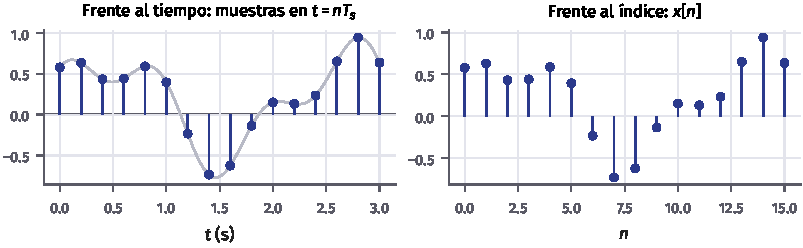
\includegraphics[width=0.64\linewidth]{muestreo_periodico}\end{center}
  \nota{La secuencia no guarda $T_s$: los mismos números representan señales distintas según la frecuencia de muestreo con que se interpreten.}
\end{frame}

\begin{frame}{Frecuencia continua y frecuencia discreta}
  Muestreamos una sinusoide $x(t)=\cos(\omega_0t+\phi)$ con periodo $T_s$:
  \[
    x[n]=\cos(\omega_0T_sn+\phi)=\cos(\Omega_0n+\phi),\qquad
    \boxed{\Omega_0=\omega_0T_s=2\pi\frac{f_0}{f_s}}
  \]
  \begin{itemize}\small
    \item La frecuencia discreta (rad/muestra) es la continua \alert{normalizada} por la frecuencia de muestreo: $F_0=f_0/f_s$ ciclos por muestra.
    \item En el T1 vimos que $\Omega_0$ y $\Omega_0+2\pi k$ dan la misma secuencia. Por tanto, todas las frecuencias continuas
    \[
      \omega_k=\omega_0+k\,\omega_s,\qquad k\in\Z
    \]
    producen \alert{exactamente las mismas muestras}.
  \end{itemize}
  \begin{importante}[Aliasing]
    Infinitas señales continuas generan la misma secuencia al muestrearlas con periodo $T_s$: cada una es un \emph{alias} de las demás.
  \end{importante}
\end{frame}

\begin{frame}{Aliasing en sinusoides}
  \begin{center}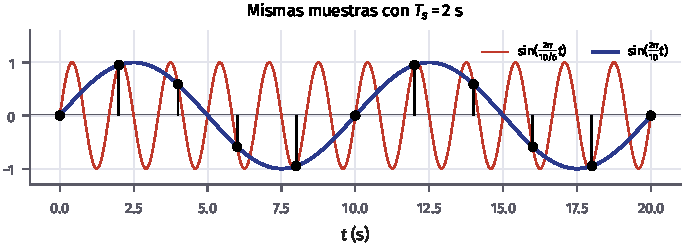
\includegraphics[width=0.78\linewidth]{alias_sinusoides}\end{center}
  \begin{itemize}\small
    \item Como el coseno es par, también $-\omega_0+k\omega_s$ da las mismas muestras: los alias son $\pm\omega_0+k\omega_s$.
    \item \alert{Alias fundamental}: el de menor frecuencia, el único con $\abs{\Omega}\le\pi$, es decir, $\abs{\omega}\le\omega_s/2$.
    \item Si $\abs{\omega_0}>\omega_s/2$, hay una sinusoide de frecuencia menor con las mismas muestras y, al reconstruir, \alert{obtenemos esa y no la original}.
  \end{itemize}
  \herramienta{T2-aliasing}
\end{frame}

\begin{frame}{Ejemplos de aliasing}
  \small
  Con $T_s=2$\,s, \ $x[n]=\sin(\omega_0T_sn)$ y el alias fundamental se obtiene llevando $\Omega_0=\omega_0T_s$ a $[-\pi,\pi)$:
  \begin{columns}[T]
    \begin{column}{0.48\textwidth}
      \begin{ejemplo}[Una sinusoide]
        \footnotesize
        $\sin\big(\frac{2\pi}{10}t\big)$: $\Omega_0=\frac{4\pi}{10}<\pi$. Ya es el alias fundamental.\\[1mm]
        $\sin\big(\frac{2\pi}{10/6}t\big)$: $\Omega_0=\frac{24\pi}{10}>\pi$.\\
        $\frac{24\pi}{10}-2\pi=\frac{4\pi}{10}$, \ $\omega=\frac{4\pi/10}{T_s}=\frac{2\pi}{10}$.\\[1mm]
        Las dos dan las mismas muestras (figura anterior).
      \end{ejemplo}
    \end{column}
    \begin{column}{0.5\textwidth}
      \begin{ejemplo}[Suma de sinusoides]
        \footnotesize
        $x(t)=3\sin\big(\frac{2\pi}{5}t\big)+\sin\big(\frac{2\pi}{3}t\big)$\\[1mm]
        $\Omega_1=\frac{4\pi}{5}<\pi$: se conserva.\\
        $\Omega_2=\frac{4\pi}{3}>\pi$: \ $\frac{4\pi}{3}-2\pi=-\frac{2\pi}{3}$, \ $\omega=-\frac{\pi}{3}$\,rad/s.\\[1mm]
        Alias fundamental:
        \[
          3\sin\big(\tfrac{2\pi}{5}t\big)-\sin\big(\tfrac{\pi}{3}t\big)
        \]
        \gris{Una frecuencia negativa en un seno cambia su signo.}
      \end{ejemplo}
    \end{column}
  \end{columns}
\end{frame}

\begin{frame}{Frecuencia aparente}
  \begin{center}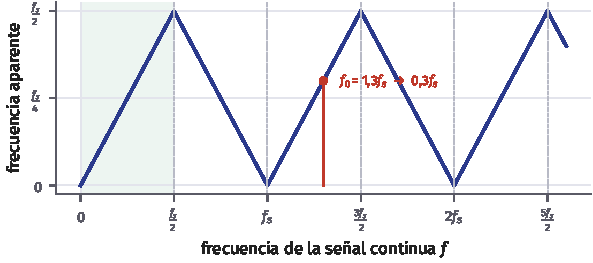
\includegraphics[width=0.6\linewidth]{alias_mapa}\end{center}
  \begin{itemize}\small
    \item Una sinusoide de frecuencia $f_0$ muestreada a $f_s$ aparece en la frecuencia
      \[f_a=\abs{f_0-k f_s}\in[0,f_s/2],\qquad k=\text{el entero más próximo a }f_0/f_s.\]
    \item El eje de frecuencias «se pliega» en múltiplos de $f_s/2$, la \alert{frecuencia de Nyquist}.
    \item Ejemplos cotidianos: las ruedas que parecen girar al revés en un vídeo, o un tono de 30\,kHz grabado a 48\,kHz que suena a 18\,kHz.
  \end{itemize}
\end{frame}

\begin{frame}{En código: alias fundamental}
  \codigo{alias_fundamental}
  \nota{\texttt{(Ω + π) mod 2π − π} lleva cualquier frecuencia discreta al intervalo $[-\pi,\pi)$.}
\end{frame}

% =====================================================================
\section{Análisis en frecuencia del muestreo}

\begin{frame}{Modelo del muestreo con un tren de impulsos}
  \begin{center}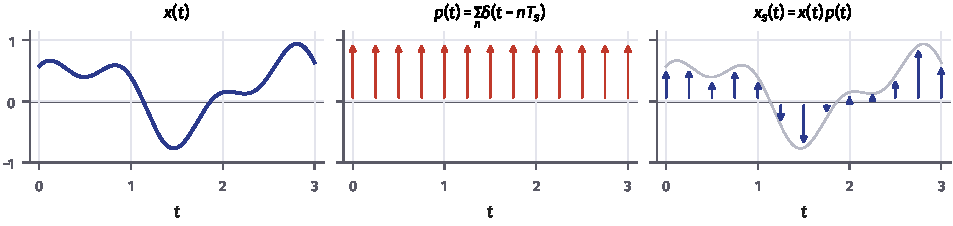
\includegraphics[width=0.92\linewidth]{tren_impulsos}\end{center}
  \[
    x_s(t)=x(t)\,p(t)=\sum_{n=-\infty}^{\infty}x(nT_s)\,\delta(t-nT_s),\qquad p(t)=\sum_{n=-\infty}^{\infty}\delta(t-nT_s)
  \]
  \begin{itemize}\small
    \item Por la propiedad del producto con $\delta$, cada impulso queda ponderado por una muestra.
    \item $x_s(t)$ es una señal de \alert{tiempo continuo} que contiene exactamente la información de $x[n]$: nos permite comparar espectros con la transformada de Fourier continua.
  \end{itemize}
\end{frame}

\begin{frame}{Transformada de Fourier del tren de impulsos}
  \begin{itemize}
    \item $p(t)$ es periódica de periodo $T_s$. Sus coeficientes de Fourier son
    \[
      c_k=\frac{1}{T_s}\int_{-T_s/2}^{T_s/2}\delta(t)\,\e^{-jk\omega_st}\dd t=\frac{1}{T_s}\quad\forall k.
    \]
    \item Una señal periódica tiene transformada $\displaystyle\sum_k2\pi c_k\,\delta(\omega-k\omega_s)$. Por tanto:
  \end{itemize}
  \begin{importante}[El tren de impulsos se transforma en otro tren de impulsos]
    \[
      \sum_{n=-\infty}^{\infty}\delta(t-nT_s)\ \parF\ \omega_s\sum_{k=-\infty}^{\infty}\delta(\omega-k\omega_s)
    \]
    Impulsos separados $T_s$ en el tiempo $\leftrightarrow$ separados $\omega_s=2\pi/T_s$ en frecuencia.
  \end{importante}
\end{frame}

\begin{frame}{Espectro de la señal muestreada}
  Por la propiedad del producto, $X_s(j\omega)=\frac{1}{2\pi}\big(X\conv P\big)(j\omega)$, y convolucionar con un impulso desplaza:
  \begin{columns}[c]
    \begin{column}{0.42\textwidth}
      \begin{importante}[Escalado y réplica]
        \[
          X_s(j\omega)=\frac{1}{T_s}\sum_{k=-\infty}^{\infty}X\big(j(\omega-k\omega_s)\big)
        \]
        El espectro se escala por $1/T_s$ y se replica cada $\omega_s$.
      \end{importante}
      {\small Si $\omega_s$ es pequeña, las réplicas se solapan y se suman: \alert{aliasing} en frecuencia.}
    \end{column}
    \begin{column}{0.56\textwidth}
      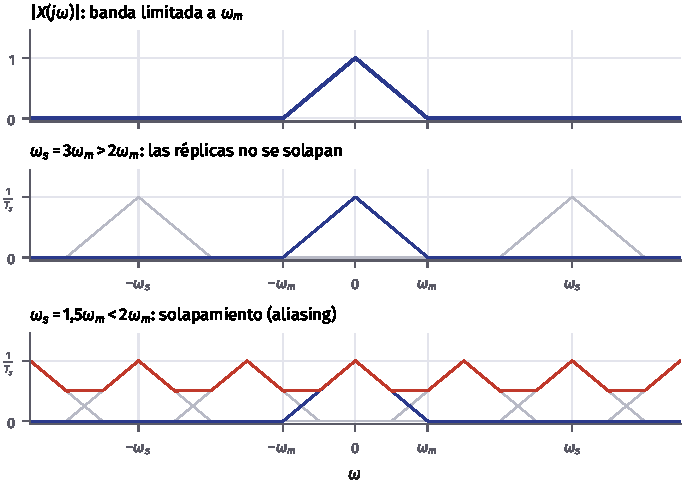
\includegraphics[height=0.66\textheight]{espectro_replicas}
    \end{column}
  \end{columns}
\end{frame}

\begin{frame}{Teorema del muestreo}
  \begin{itemize}
    \item Si $X(j\omega)=0$ para $\abs{\omega}>\omega_m$, la réplica $k$ ocupa $[k\omega_s-\omega_m,\ k\omega_s+\omega_m]$.
    \item Las réplicas $0$ y $1$ no se solapan si $\omega_m<\omega_s-\omega_m$.
  \end{itemize}
  \begin{definicion}[Teorema de Nyquist–Shannon]
    Una señal de \alert{banda limitada}, con $X(j\omega)=0$ para $\abs{\omega}>\omega_m$, queda determinada por sus muestras si
    \[
      \omega_s>2\,\omega_m\qquad\big(f_s>2f_m\big).
    \]
  \end{definicion}
  \begin{itemize}\small
    \item $2f_m$ es la \alert{tasa de Nyquist}; $f_s/2$ es la \alert{frecuencia de Nyquist}.
    \item La desigualdad debe ser estricta: $\sin(\omega_mt)$ muestreada a $\omega_s=2\omega_m$ da $\sin(\pi n)=0$ en todas las muestras.
    \item Si no se cumple, las réplicas se solapan y la señal original \alert{no se puede recuperar}.
  \end{itemize}
  \herramienta{T2-muestreo-ideal}
\end{frame}

\begin{frame}{Visión continua y visión discreta del muestreo}
  Transformando $x_s(t)$ término a término:
  \[
    X_s(j\omega)=\sum_{n}x(nT_s)\,\e^{-j\omega T_sn}
    \qquad\text{y la DTFT de }x[n]\text{ es}\qquad
    X(\e^{j\Omega})=\sum_{n}x[n]\,\e^{-j\Omega n}.
  \]
  \begin{importante}[Relación entre las dos frecuencias]
    \[
      X(\e^{j\Omega})=X_s(j\omega)\big|_{\omega=\Omega/T_s}=\frac{1}{T_s}\sum_{k=-\infty}^{\infty}X\Big(j\,\frac{\Omega-2\pi k}{T_s}\Big),\qquad \Omega=\omega T_s
    \]
  \end{importante}
  \vspace{-1mm}
  \begin{center}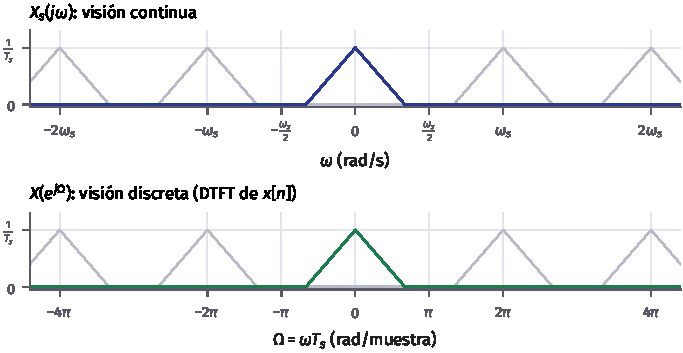
\includegraphics[height=0.31\textheight]{vision_continua_discreta}\end{center}
\end{frame}

\begin{frame}{Consecuencias de $\Omega=\omega T_s$}
  \begin{itemize}
    \item El intervalo $\abs{\omega}\le\omega_s/2$ se transforma en $\abs{\Omega}\le\pi$: toda la información útil de la señal muestreada está en una banda de anchura $2\pi$.
    \item La periodicidad $2\pi$ de la DTFT \alert{es} la replicación del espectro causada por el muestreo.
    \item Con $\omega_s=2\omega_m$ la banda $[-\pi,\pi]$ está completamente ocupada. Con \alert{sobremuestreo}, por ejemplo $\omega_s=4\omega_m$, la señal ocupa $\abs{\Omega}\le\pi/2$ y queda un margen libre que facilita el filtrado.
  \end{itemize}
  \begin{ejemplo}[Una frecuencia en tres unidades]
    Un tono de $f_0=1$\,kHz muestreado a $f_s=8$\,kHz: \ $\omega_0=2\pi\cdot1000$\,rad/s, \ $F_0=1/8$ ciclos/muestra, \ $\Omega_0=\pi/4$\,rad/muestra.
  \end{ejemplo}
\end{frame}

\begin{frame}{En código: espectro de una señal muestreada}
  \codigo{espectro_muestreado}
  \nota{Representar $T_s\abs{X(\e^{j\Omega})}$ frente a $\omega=\Omega/T_s$ deshace el escalado y permite comparar con $X(j\omega)$.}
\end{frame}

% =====================================================================
\section{Muestreo en la práctica}

\begin{frame}{Filtro antialiasing}
  \begin{center}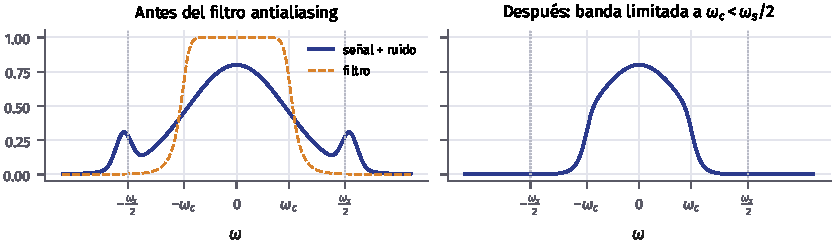
\includegraphics[width=0.8\linewidth]{antialiasing}\end{center}
  \begin{itemize}\small
    \item Las señales reales no tienen banda limitada: una señal de duración finita tiene espectro infinito, y el ruido ocupa todas las frecuencias.
    \item El filtro analógico antialiasing elimina lo que está por encima de $f_s/2$ \alert{antes} de muestrear: después ya no hay forma de separarlo.
    \item Como un filtro real no corta en seco, se muestrea con margen: el CD usa $f_s=44{,}1$\,kHz para audio de 20\,kHz.
  \end{itemize}
\end{frame}

\begin{frame}{Muestreo no ideal}
  \begin{center}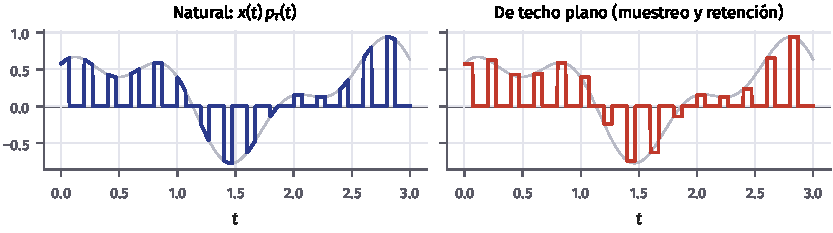
\includegraphics[width=0.8\linewidth]{muestreo_natural}\end{center}
  \begin{itemize}\small
    \item Los impulsos ideales no existen: se muestrea con pulsos de duración $\tau$.
    \item \alert{Natural}: $x(t)\,p_\tau(t)$. Las réplicas no se deforman, solo se ponderan con los coeficientes del tren de pulsos.
    \item \alert{De techo plano}: cada pulso mantiene el valor de la muestra (es lo que hace el \emph{sample and hold}). Equivale a $x_s(t)$ convolucionada con un pulso, así que el espectro se multiplica por un $\sinc$: \alert{efecto de apertura}, el mismo del retenedor de orden cero (parte 2).
  \end{itemize}
  \herramienta{T2-muestreo-natural}
\end{frame}

% =====================================================================
\section*{Resumen}
\begin{frame}{Conceptos importantes}
  \begin{columns}[T]
    \begin{column}{0.5\textwidth}
      \begin{itemize}
        \item Cadena de procesado: antialiasing, A/D, procesado, D/A, reconstrucción.
        \item Muestreo, cuantificación y codificación.
        \item $x[n]=x(nT_s)$ y $\Omega=\omega T_s$.
        \item Aliasing: $\omega_0$ y $\omega_0+k\omega_s$ dan las mismas muestras. Alias fundamental en $\abs{\omega}\le\omega_s/2$.
      \end{itemize}
    \end{column}
    \begin{column}{0.5\textwidth}
      \begin{itemize}
        \item El muestreo escala el espectro por $1/T_s$ y lo replica cada $\omega_s$.
        \item \alert{Nyquist–Shannon}: $\omega_s>2\omega_m$.
        \item Filtro antialiasing antes del A/D.
        \item Muestreo natural y de techo plano.
      \end{itemize}
    \end{column}
  \end{columns}
  \bigskip
  \gris{Apuntes del Tema 2, secciones 1–3 · Hoja de ejercicios, ejercicios 1–6.}
\end{frame}

\end{document}
